
\documentclass[a4paper,11pt]{report}
%This is a comment
%USED PACKAGES
\usepackage[utf8]{inputenc}  %Fixd #inputencoding
\usepackage[italian]{babel}
\usepackage[T1]{fontenc} % encoding del font
\usepackage{amsfonts} % fonts matematici
\usepackage{amsmath} % estensione di amsfonts
\usepackage{indentfirst}
\usepackage{eurosym}
\usepackage{graphicx}
\usepackage{dirtytalk}
\usepackage{epigraph}

\newtheorem{theorem}{Theorem}
%PREAMBLE
\hyphenation{Maturity}
\hbadness=99999 %rimuove warning di bruttezza

\title{ Business Intelligence for Financial Services}
\author {Leonardo Fraquelli }

\begin{document}
\maketitle
%This is a test for commands and is not part of the full text
%\%newline
%\TeX
%{\bfseries Questo sar\'a del testo in grassetto BOLD }   % \textbf{testo} too
%{\rmfamily Questo sarà del testo in roman}
{%\bfseries Queste funzioni \emph { possono contenere altre funzioni }}
% I seguenti comandi: \newline \newpage  interrompono il testo e vanno a capo
% \hspace{} \vspace inseriscono spazi orizzontali/veritcali, VANNO ESPRESSI CON UNITA DI MISURA

% part,chapter,section,subsection,subsubsection sezionano il documento 
% part>chapter>section...

%footnote inserisce una nota numerata a fine pagina
%marginpar[testosx]{testodx} è una nota a margine NOTA LA DIFFERENZA { [

%  \section{riferimenti} \label{Tipo:nome} fa in modo che una sezione possa essere riferita attraverso il comando
%  \ref{Tipo:nomei}
%sillabazione   \hypenation{co-me vuoi sil-la-ba-re una parola}  ESEGUI QUESTO DURANTE LA REVISIONE DEL TESTO
\part{Concetti base di Finanza}

\chapter{Financial Instruments}
Gli strumenti finanziari utilizzati in questo corso rientrano in una grossa categoria chiamata {\bfseries Securities} \newline
{\bfseries Securities}: sono uno strumento negoziabile che {\bfseries rappresenta un valore finanziario.} \newline
Questi sono: 
\begin{description}    %begin itemize consente di fare liste "Ad albero" con rientranze che aumentano per ogni itemize effettuato

\item[Debt]: sono securities che sono considerate \textbf{risk-free} \footnote{Queste sono lo standard(benchmark) di riferimento per considerare poi il guadagno di stocks rispetto ad altre securities}
\item[Equity]: sono le \textbf{Stocks (Azioni)} di una compagnia
\item[Derivatives]: sono securities il cui valore dipende da più variabili. \\ Queste sono: \bfseries {futures, forwards, swaps, options}
\end{description}
Le Securities sono, in genere, scambiate a un exchange market, un mercato finanziario. \newpage

%%%% NEWPAGE
\section{Computing profit}
è bene definire un paio di termini:
\begin {description}
\item[Bond] è un contratto a lungo termine tra due soggetti.
\item[Issuer] è il debitore: riceve X soldi dall' {\bfseries Holder} ed è obbligato a ripagarli in seguito con degli {\bfseries Interessi}.
\item[Holder] è il creditore: "Presta" X soldi all' {\bfseries Issuer} e viene ripagato in seguito.
\item[Principal] è l'ammontare iniziale di soldi che {\bfseries l'Holder} rilascia.
\item[Coupons] sono i successivi interessi sulla {\bfseries Principal}.
\item[Maturity Date] è la data in cui il {\bfseries Bond} termina.
\end {description}
Il valore di un bond dipende quindi da:  {\bfseries Il tempo di maturità, gli interessi e la frequenza di pagamento}. \newline
Supponendo di avere un investitore che acquisisce un bond con: \newline
\textbf{Principal}=100\euro \newline
\textbf{interesse annuale}=10\% \newline
Allora il valore del bond dopo un anno sarà: \newline
 100\euro+(0.1*100 \euro)= 100 \euro *(1+0.1)=110 \euro
\newpage

%%%% NEWPAGE
\subsection{Compounding of Interest Rates}
La seguente formula considera: 
\begin{align*}
P &= \text{principal (i-esima) con $P_0$ = principale} \\
n &= \text{numero di anni}\\
r &= \text{tasso di interesse annuale}\\
\end{align*}
Ed è la \textbf{Formula generica per il compounding dei tassi di interesse} 
\begin{center}
 $P_n=P_0*(1+r)^n$ t \newline
Aumentando la frequenza di pagamenti (e.g. con interessi semestrali) la formula diventa: \newline
 $P_n=P_0*(1+{\frac {r}{m}})^{\frac{n}{m}} $ \newline
\end{center}
\begin{figure}[h!]
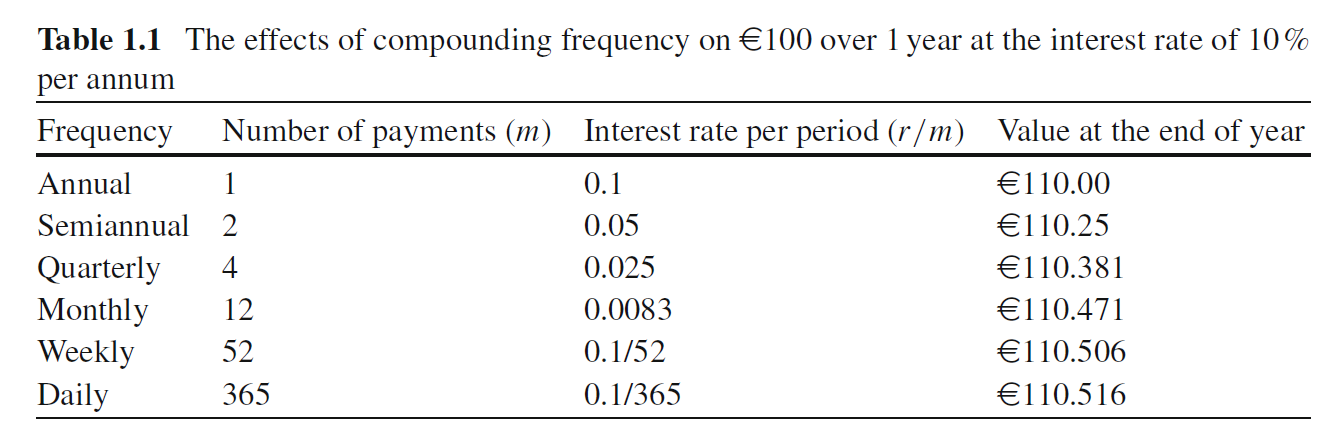
\includegraphics[width=\linewidth]{TableInterests.png}
\caption {Tabella raffigurante la crescita dei valori al crescere di m}
\end{figure}
\newpage

%%%% NEWPAGE
\section {Payoff e profit dei bond}
il \textbf{Payoff} di una security è il suo valore al raggiungimento della  \textbf{Maturity } 
Per i \textbf{Bond} il payoff nient'altro è che \textbf{Principal + Interessi} \newline
Il \textbf{Profitto} di una security è il \textbf{payoff aggiustato}, rimuovendo l'investimento iniziale,tasse ed altri costi di transazione. \newline
Per I \textbf{Bond} non vi sono tasse o costi aggiuntivi, diciamo quindi che il rischio è \textbf{NULLO}
\newline \textbf{Formula per il calcolo del profitto ad un tempo $\tau$} \newline
{\LARGE {$P_\tau - P_0 = P_0*((1+{\frac {r}{m}})^{m*\tau}-1)$}}
\subsection{Continous Compounding}
Aumentando nelle precedenti formule \textbf{m} ad infinito otteniamo il \textbf{Continous Compounding} \newline
Assumiamo quindi che il valore di una security aumenti continuamente in un periodo di tempo \textbf{t>0}\newline
La nuova formula diventa: \newline
{\LARGE {$P_\tau = P_0*e^{r*\tau}$}}
\newpage

%%%% NEWPAGE
\section{Stocks: Trade, Price, Indices}
Le \textbf{Stocks} sono una parte dell'asset e dei guadagni di una compagnia \newline
Possono Essere di due tipi
\begin{description}
\item[Common] Generalmente concedono al proprietario uno share dei dividendi e il voto ai meeting degli shareholder
\item[Preferred] Consentono solamente una \textbf{priorità} nel ricevimento dei dividendi
\end{description}
Una compagnia vende Stocks(Shares) per aumentare il capitale attraverso degli Exchange market \newline
Negli Exchange market un \textbf{broker} sarà il responsabile delle operazioni
questo consente di calcolare la \textbf{capitalizzazione o MarketValue} di una compagnia \newline
\begin{center}
\textbf{MarketValue =} numero di share  * prezzo di una share
\end{center}
Questo Valore varia nel tempo.
\subsection {Compravendita di stocks}
Negli Exchange market sono eseguiti ordini di \textbf{buy} e di \textbf{sell} \newline
questi sono eseguiti attraverso \textbf{orders} di diverso tipo, che consentono di avere delle \textbf{trading strategies}\newline
Tali orders sono detti:
\begin{description}
\item[Market Order:] Sono ordini da eseguire IMMEDIATAMENTE al prezzo migliore \newline  \begin{itemize} 
	 %reference a grafo dei prezzi?
	 \item Utilizzati se l'esecuzione dello scambio ha priorità sul prezzo
 	 \item Prendono il miglior prezzo possibile (fill price) al momento dell'esecuzione {\footnote{Può variare quindi rispetto al prezzo mostrato}}
	\end{itemize}
\item[Limit Order] Inviati al mercato per scambiare solo da un prezzo predefintio \newline \begin{itemize}
	\item Lo scambio è eseguito solo se(quando) vi è un offerta valida
	\item Questo tipo di ordine da controllo sul prezzo ma non sul tempo
	\end{itemize}
\item[Stop Order] Un ordine mantenuto dal broker e non inviato sul mercato finchè non viene raggiunto un certo prezzo \newline \begin{itemize}
	\item Quando il prezzo è raggiunto lo stop-order può diventare un market o limit order \footnote{Specificato dall'investitore}
	\item Può limitare le perdite 
	\item A differenza del limit order lo stop order non è inviato al mercato immediatamente \footnote{Come scegliere il prezzo 		dello stop order è topic di ricerche}
\end{itemize}
\end{description}
Utili provider di quote sulle azioni sono Yahoo Finance e Google Finance (Yahoo>Google ) \newpage

%%%% NEWPAGE

\section{Storico transazioni}
	Per questa sezione faremo riferimento a YahooFinance \newline
	Nella lettura delle quote di una Azienda particolare sono presenti i seguenti TAG \newline
\begin{description}
	\item[Ticker] L'id dell'azienda (AAPL=> Apple Inc.)
	\item[Open] Il prezzo delle share dell'azienda all'apertura del mercato
	\item[Close] Il prezzo attuale, se il mercato è aperto, il prezzo di chiusura altrimenti
	\item[High] Massimo prezzo raggiunto tra Open e Close
	\item[Low] Minimo prezzo raggiunto tra Open e Close
	\item[Adjusted Close] il prezzo di Close aggiustato includendo dividendi ed altre azioni che possono aver modificato il prezzo
	\item[Volume] quantità di shares scambiate (non viene precisato se buy/sell)
	\item[Dividend] un pagamento periodico che riflette i profitti in ritorno agli shareholder
\end{description}
è possibile che alla chiusura e all'apertura del mercato Open e Close del giorno precedente non coincidano \newline
questo perchè alcuni scambi potrebbero alterare il valore in chiusura %%%Not important
\newpage

%%%%NEWPAGE

\section{Payoff e profit delle stocks}
	Verranno utilizzate le seguenti variabili:
\footnote {this is not full, please send help}
\begin{align*} %%aggiungi le prossime variabili
	S &= {\text {prezzo della stock S al tempo T con $S_0$= prezzo iniziale}}\\
	T &= {\text {tempo con $S_T$ = tempo di vendita}}\\
	r &= {\text { tasso di interesse}}\\
\end{align*}
\begin{center}
	$S_\tau + D_\tau - C(S_0)e^{r*\tau}$
\end{center}
%\newline
\section{Stock Indices} \label{Indici:1}
Un \textbf{indice} è una funzione matematica che misura i cambiamenti in un gruppo di \textbf{data points} \newline
Negli Exchange market questi indici sono i cambiamenti nel valore di un gruppo selezionato di stocks \newline
Sono un riferimento generale per il trend del mercato e dell'economia \newline
Sono ovviamente non acquistabili \newline
Gli indici possono essere di diversi tipi
\begin{description}
	\item[Price weighted] considerano il prezzo dei componenti delle stock che compongono l'indice
	\item[Capitalization weighted] considerano il prodotto prezzo*quantita di ogni stock che compone l'indice
\end{description}
L'importanza degli indici sta nel poter misurare la performance degli investimenti in un determinato gruppo di azioni rispetto ad altri \newline
In particolare il confronto tra i\textbf{rate of Benefit cumulati} che si ottengono durante l'investimento \newline
Per una serie di prezzi $P_t$ con t>=0 il \textbf{rate of benefit o ritorno} è \newline
\begin{center}
	$R_t=({\frac{P_t}{P_{t-1}}})-1$
\end{center}
i ritorni verranno analizzati più tardi %% Reference pls
\newpage
\section{Opzioni e Derivate}
	Un \textbf{Opzione} è un contratto tra investitori nel quale si acquista \textbf{l'opportunità} ma non \textbf{l'obbligo} 
	di scambiare un particolare asset in una data futura ad un prezzo prestabilito \newline
	Termini: \newline
\begin{description}
	\item[Exercise date o Maturity:] data prestabilita in cui verrà svolto lo scambio 
	\item[Exercise o Strike price:] prezzo dell'asset che viene prestabilito
	\item[Call/Put:] il tipo di \textbf{Opzione}, ovvero di \textbf{acquisto/vendita}
	\item[Esercitare l'opzione] Effetturare lo scambio
\end{description} 
	Le opzioni possono essere di diversi tipi:
\begin{description}
	\item[Vanilla] Sono Opzioni classiche, caratterizzate solo da condizioni dirette di payoff
		\begin{itemize}
			\item \textbf{Europee} possono essere esercitate solamente alla maturity
			\item \textbf{Americane} possono essere esercitate qualunque giorno prima della maturity
		\end{itemize}
	\item[Exotic] Hanno condizioni più complesse
		\begin{itemize}
			\item \textbf{Bermudane} possono essere esercitate in date predeterminate
		\end{itemize}
	\item[Path-dependent] hanno un payoff che dipende dalla loro price history
		\begin{itemize}
			\item \textbf{Asiatiche} hanno un payoff determinato dalla media del prezzo durante la vita dell'opzione
			\item \textbf{A Barriera} posono essere esercitate solo se il prezzo sorpassa un certo livello in un periodo di tempo
		\end{itemize}
\end{description}
	Il prezzo di una opzione è chiamato \textbf{premio} ed è dato per \textbf{ogni} azione
	 \footnote{questo vuol dire che comprando un premio di  \EUR{1.00} ad un predeterminato prezzo X per N azioni pagherò $N*(X+1.00)$}
	\newline  Le opzioni sono organizzate in "serie" di differenti premi, per una maturity date e quotate agli exchange market nel 		seguente modo \newline
\begin{center}
	SecuritySymbol + ExpirationDate + Type(Call/Put) + StrikePrice
\end{center}
\section{Payoff e Profit delle opzioni}
	Il payoff di una opzione dipende dalla possibilità di esercitarla o meno
\begin{align*}
	\text{$P_T$} &= \text{Prezzo di un asset alla data T} \\
	K &= \text{Strike Price alla data T} \\
\end{align*}
	il payoff di un contratto call generico sarà
\begin{center}	
	max($P_T$ - K, 0) \footnote{ esercitiamo solo se $P_T$ > K}
\end {center}
	il payoff di un contratto put generico sarà
\begin{center}	
	max(K - $P_T$ , 0) \footnote {esercitiamo solo se $P_T$ < K}
\end {center}
	il payoff delle opzioni path dependent è dipendente dalle diverse condizioni sullo strike price \newline
\subsection {Profit delle opzioni}
	Per computare il profitto delle opzioni dobbiamo considerare la commissione data \footnote{il prezzo della opzione}
\begin{align*}
	\text{$P_0$} &= \text{prezzo dell'asset al tempo $T_0$} \\
	T &= \text{tempo settato per la maturity} \\
	\text{C($P_0$,T)} &= \text{il prezzo ottenuto dalla coppia P,T}\\
\end{align*}
in questo caso sottraiamo il prezzo dell'opzione dal payoff, ma considerato che questi valori sono ricevuti a un diverso periodo T dobbiamo includere i possibili guadagni che avremmo ricevuto con un asset risk-free con in tasso di investimento r\footnote{ $\tau$ = T-$T_0$} \newline

\begin{center}
	$max(P_T - K, 0) - C(P_0,T)e^{r*\tau}$
\end{center}
\subsection{Perchè le opzioni}
	utilizzare delle opzioni dà 2 vantaggi rispetto all'acquisto diretto di azioni
\begin{enumerate}
	\item Possiamo riservare un acquisto di più azioni pagando solo il premio
	\item Questo, di per se pone un limite sulle perdite
\end{enumerate}
\subsection{Prezzatura delle opzioni}
	In un contratto opzione entrambi i partiti assumono un rischio:
\begin{enumerate}
	\item \textbf{L'Holder} assume un rischio pagando il premio, che sarà una perdita se non esercita la opzione
	\item \textbf{L'Issuer} assume un rischio, in quanto se l'opzione viene esercitatà sarà a un prezzo minore del prezzo di 	mercato
\end{enumerate}
\newpage

%%%% NEWPAGE
\section{Futures and Forwards}
	I \textbf{Futures ed I Forwards} sono \textbf{Derivate}, differiscono dalle opzioni per l'essere un \textbf{OBBLIGO} \newline
	Due gruppi creano un contratto con l'obbligo di scambio di uno specifico asset, per un prezzo \textbf{delivery price} e una 		data specifica (\textbf{Forwards}) o periodo di tempo (\textbf{Futures}). \newline
	L'asset scambiato può essere una \textbf{commodity}(qualsiasi cosa) \newline
	I contratti forward non sono scambiati negli exchange market
\subsection{Payoff e Profit di Futures and Forwards}
	Profit e payoff sono uguali in quanto questi contratti non includono fee, \newline
	siano:
\begin{align*}
	K &= \text{prezzo del delivery price dell'asset}\\
	\text{$P_T$} &= \text{Prezzo dell'asset al tempo T} \\
\end{align*}
	allora il profit/payoff è
\begin{center}
	$P_T$-K  \small{per l'acquisto} \\
	K-$P_T$ \small{per la vendita}
\end{center}
\newpage

%%%% NEWPAGE
\section{Portfolio}
\begin{description}
	\item[Portfolio:] collezione di una o più securities da un investitore, o da una compagnia
	\item[Positions:] gli elementi di un portfolio
	\item[Valore di un Portfolio:] la somma dei valori delle posizioni ad un dato periodo di tempo
	\item[Profit di un Portfolio:] la somma dei profit delle posizioni ad un dato periodo di tempo
\end{description}
	Un portfolio è designato e aggiornato per adeguarsi agli obbiettivi di un investitore, ai suoi risultati attesi, in continuo 			confronto con la sua tolleranza al rischio. \newline
	\textbf{Il management di un portfolio} richiede due operazioni di base
\begin{description}
	\item[Apertura di una posizione] aumenta i risultati attesi aggiungendo una nuova posizione
	\item[Chiusura di una posizione] riduce il rischio di decrescere il valore del portfolio vendendo una posizione
	\item[Allocare degli asset:] sono le dinamiche dell'apertura e della chiusura al fine di minimizzare il rischio e massimizzare i 		profitti
\end{description}
\subsection{ETF e Fondi mutuali}
	Invece di gestire personalmente un portfolio è possibile investire su un portfolio collettivo di una compagnia professionale \newline
	La compagnia decide le securities, le loro performance, e esegue allocazioni di asset al posto dell'individuo. \newline
	I \textbf{Fondi mutuali (?)} sono lo strumento di investimento collettivo più comuni:
\begin{enumerate} %Swtich a una lista non numerata 
	\item Sono regolati e registrati ad un exchange market	 
	\item Sono pubblici
	\item possono essere \textbf{Closed-end} ovvero con un numero fisso di azioni
	\item oppure \textbf{Open-end} senza limiti al numero di share, che l'investitore può vendere ad ogni momento, uscendo dal 	fondo
\end{enumerate}
	Un altro tipo di investimento collettivo è un \textbf{ETF}, Exchange-traded Fund \newline
	simile a un fondo closed-end ma gestito da uno stock exchange \newline
	Molti ETF sono costruiti per tracciare uno specifico indice % \ref{Indici:1}

\newpage

%%%% NEWPAGE
\chapter{Trading}
\section{Posizioni di Trading}
	\textbf{Posizioni lunghe e corte}
	Un investitore che possiede una security è detto \textbf{long} nella security \newline
	Un investitore che "presta" una security è detto \textbf{short} nella security \newline
	L'atto di acquisto/vendita è detto assumere una \textbf{long/short} position  \newline
	Per trovarsi in short un broker deve decidere di prestarci la security, per poi venir ripagato in seguito \newline
	Queste operazioni sono dette \textbf{short selling} e sono molto spesso illegali

\newpage

%%%% NEWPAGE
\section{Trading Attitudes}
	consideriamo tre tipi particolari di traders:
\begin{description}
	\item[Hedgers] eseguono scambi riducendo o eliminando il rischio quando prendono una posizione su una security \footnote{ 		Si mantengono sul "bordo" del mercato"}
	\item[Speculators] eseguono scambi rischiosi, scommettendo sul futuro prezzo di una security
	\item[Arbitrageurs] eseguono scambi \footnote{legali?} che sono avvantaggiati su più mercati
\end{description}
\subsection{Hedgers}
	scambi \textbf{risk-free}, \newline
	Loro scopo è proteggere il portfolio dalla perdita di valore, con un compromesso sui benefit possibili.\newline
	Una strategia di Hedging generalmente acquista share con posizioni inverse\footnote{Quando una sale, l'altra scende} in 			modo tale da compensare la decrescita di una con la crescita dell'altra.
\subsection{Speculators}
	scambi \textbf{basati su speculazione}, sono una scommessa sul futuro prezzo della security.
\subsection{Arbitrageurs}
	scambi \textbf{fra diversi mercati}, scambiano su mercati vantaggiosi e riscambiano gli acquisti su mercati a prezzi più alti \newline
	cercano degli sbilanci fra i prezzi di due mercati.
\subsubsection{L'arbitraggio}
	generalmente parlando, i costi di transazioni riducono considerabilmente il profitto, e nel caso di grosse disparanze nei prezzi 		altri trader se ne accorgeranno subito, diciamo quindi che le possibilità di arbitraggio sono praticamente nulle.
\newpage
\section{Bulls/Bears} %...
	Quando il trend del mercato è in crescita\footnote{vedi indici}, si dice che è "bullish" \newline
	Quando il trend del mercato è in decrescita, si dice che è "bearish" \newline
	un \textbf{Bull, o Toro,} è un investitore che prende una posizione di long quando il prezzo è in crescita \newline
	un \textbf{Bear, o Orso,} è un investitore che prende una posizione di short quando il prezzo è in decrescita. \newline
\emph{\say{When the market is bullish assume long positions, when bearish assume short positions.}}
\subsection{Determining bull or bear}
	Determinare se il mercato è bullish/bearish nient'altro è che determinare la crescita futura e la sua sostenibilità, \newline
	Questo richiede moltissime variabili. \newline
	Una definzione accettabile di un mercato bearish è: 

\emph{\say{While there's no agreed-upon definition of a bear market, one generally accepted measure is a price decline of 20\% or more
	over at least \textbf{a two-month period}}}

\section{Market Timing}
	un \textbf{atteggiamento passivo} è quello che la maggioranza degli investitori segue, consiste in una strategia detta 				\textbf{buy and hold} nella quale le securities sono mantenute in un portfolio per un lungo periodo di tempo.

	La motivazione è che in genere ogni security tende ad aumentare di prezzo con il passare del tempo.

	D'altro canto se osserviamo il trend di crescita/decrescita viene naturale chiedersi se non sarebbe meglio vendere ai massimi e 	comprare ai minimi.
\subsection{Strategie di Timing}
	Esistono diversi metodi per sviluppare delle strategie, queste includono l'utilizzo di modelli per prevedere i ritorni %ref ai ritorni chapt1
	analisi strutturali dei prezzi e fondamenti dell'economia di mercato...

	Per una qualunque strategia, ci si aspetta che possa battere i risultati ottenuti di chi effettua trading senza alcuna strategia
\section{Prezzo vs Valore}
	Non vi è più interesse oggi alla compagnia dietro una security, quanto il suo valore sul mercato per la maggior parte degli 		 	investitori,

	Il prezzo di un'azione riflette oggi le forze di \textbf{supply and demand}
\subsection{Modello Discounted Cash Flow}
	Il valore di una stock per un investitore dipende dai \textbf{possibili guadagni} futuri \newline
	I guadagni futuri derivano da i \textbf{dividendi} e l'eventuale \textbf{prezzo di vendita} \newline
	quindi per ottenere una stima del valore di $S_0$ nel periodo, per esempio, di un anno vanno considerati
\begin{align*}
	\text{$D_1$} &= \text{Dividendi ottenuti in un anno}\\
	\text{$S_1$} &= \text{Valore della stock in un anno}\\
	r &= \text{discount rate (?)}\\
\end{align*}
\begin{center}
	$S_0={\frac{D_1+S_1}{1+r}}$
\end{center}
	 ripetendo questo per un numero arbitrario T di anni otteniamo la seguente formula
\begin{center}
	$S_0 =\sum\limits_{t=1}^T {\frac {D_t}{(1+r)^t}}+{\frac {S_T}{(1+r)^T}}$
\end{center}	
	possiamo assumere che dopo T anni il valore di $S_T$ tenda a 0  \newline
	per questo inroduciamo il \textbf{DCF, discounted cash flow model} che rappresenta il valore di un'azione attraverso i suoi 		dividendi
\begin{center}
	$S_0 =\sum\limits_{t=1}^T {\frac {D_t}{(1+r)^t}}$
\end{center}
	Prima di fare delle stime con \textbf{DCF} dobbiamo precisare la natura di r \newline
	possiamo considerarlo come il tasso di interesse di un bond risk-free \newline
	possiamo vedere r come:
\begin{center}
	$r={\frac {D_1 + S_1}{S_0}}-1$
\end{center}
	questo ci dice che r è il ritorno %%%% SEE ref:returns
	atteso della stock, oppure potrebbe essere il ritorno di un asset simile, ma risk-free \newline
	in questo modo definiamo r come \textbf{il rate della capitalizzazione del mercato} oppure \textbf{il capitale del costo di 			equità} come interpretazioni precise di r

\newpage 

%%%% newpage
\section{Arbitraggio}
\epigraph{There is no such a thing as free lunch}{Milton Freedman } 
	Un assuzione economica sotto ogni modello matematico è che è \textbf{impossibile} avere dei profitti senza rischio \newline
	
	Questa assunzione è detta \textbf{Principle of No Arbitrage}: there are no arbitrage opportunities. \newline
	Si può espandere questo principio con altre assunzioni \newline
\subsection{Extended no arbitrage}
\begin{itemize}
	\item Non è possibile \textbf{fare} arbitraggio
	\item Nello short-selling non ci sono tasse,costi di transazione o restrizioni
	\item è possibile prestare e farsi prestare a rate d'interese risk-free
	\item Ogni security è perfettamente divisibile (?)
\end{itemize}
\subsection{Consequenze}
\begin{description}
	\item[Conseq. 1] Assumendo niente arbitraggio, due portfolio con valore uguale ad un tempo T avranno valore uguale 		$\forall$ t tali che t $\leq$ T
	\item[Conseq. 2] Assumendo niente arbitraggio, siano A,B due portfolio

	 con v(A,T)$\geq$ v(B,T) allora $\forall$ t $\leq$T questa proposizione sarà vera
\end{description}

\section{Valutazione Risk-neutral}
	Un semplice metodo di valorizzare un opzione deriva dall'assunzione che gli investitori sono indifferenti al rischio, \newline
	\textbf{la neutralità al rischio} è un ipotesi \textbf{forte}, ma è ottima per valorizzare un opzione \newline
	Ipotizzando un mondo neutrale al rischio le securities si comportano esattamente come un bond, quindi il beneficio di una stock sarà uguale a un investimento risk-free.
	il valore di una derivata può essere ottenuto calcolando il valore atteso, e rimuovendo la "spesa del rischio":
\begin{center}
	$S_T + D_\tau - C(S_0)e^{r\tau}$
\end{center}
\section{Ipotesi di mercato efficiente EMH*}
	{\tiny{Efficient Market Hypothesys*}} \newline
	Un altro paradigma interessante per valutare l'equilibrio del mercato nasce dall'assunzione che un mercato è "information efficient": \newline
	\emph{ Le informazioni disponibili al momento dell'investimento si riflettono gia nel prezzo della security, di consequenza i partecipanti al mercato non possono avvantaggiarsi delle informazioni attuali per aumentare il proprio profitto}

\subsection{Test di EMH}
	L'efficienza di \textbf{EMH} è argomento di diversi studi; \newline
	il metodo generico per testare EMH consiste di
\begin{enumerate}
	\item Designare una strategia basata su un insieme di informazioni,
	\item Misurare i ritorni rispetto un insieme senza queste informazioni
\end{enumerate}
	Per la prima parte, dobbiamo specificare l'insieme di informazioni e l'efficienza di tale \textbf{informazione}:
\begin{description}
	\item[Debole] l'informazione riguarda lo storico di prezzi della security
	\item[Semi-Forte] ogni informazione pubblica è disponibile \footnote{e.g ciò che una compagnia rilascia}
	\item[Forte] ogni informazione pubblica \textbf{e privata} è disponibile \footnote{in genere, queste informazioni hanno un prezzo, dobbiamo verificare che il costo di queste informazioni sia minore del nostro profitto}
\end{description}
	Diverse ricerche hanno dimostrato che la presenza di informazioni Forti,Semi-forti forniscono un vantaggio per i trader che 		utilizzano solamente informazioni deboli. \newline
\subsubsection{EMH e la computabilità}
	Studi recenti hanno dimostrato che un mercato può essere definito rispetot a delle risorse di computazione R
	questo vuol dire che si possono migliorare i profitti assegnando R risorse (tempo,memoria...) alla nostra strategia
	questo vuole anche dire che un vantaggio può derivare da grosse facilities, vicinanza al mercato...\footnote{Per approfondire: Michael Lewis, Flash Boys. un libro sull'HighFrequency Trading} %Sei troppo povero per questo
\newpage

%%%% NEWPAGE

%%FINE SLIDE 3

\chapter{Electronic Market, Limit Order Book}

\section{Trading nel mercato elettronico}
	Gli ordini sono gestiti da un \textbf{engine} e dal \textbf{Limit Order Book(LOB)}. \newline
	Il LOB gestisce ogni order, in entrata e in uscita

	\textbf{L'engine} utilizza degli algoritmi per definire quando uno scambio può avvenire e in tal caso, quale criterio usare per 		eseguire degli ordini

	La maggior parte dei mercati favorisce \textbf{Market Order} ai \textbf{Limit Order}, e utilizzano una priorità prezzo/tempo dove:
\begin{enumerate}
	\item L'ordine viene assegnato al miglior LO e viene eseguito(e.g compra 100 stocks a 20\$)
	\item Se l'ordine non è finito ma l'offerta di LO si, il rimanente ordine viene eseguito al prossimo migliore LO(e.g compra le rimanenti stocks a \$25)
	\item ripeti se necessario
\end{enumerate}
	I limit order che sono più "a fondo" nel \textbf{LOB} sono detti a fondo \newline
	un MO che viene eseguito ai LO "in fondo" è detto \textbf{walking the book}

	per questo esistono MO di genere \textbf{Immediate-or-Cancel} che prevengono agli ordini di andare su offerte "terribili"
\subsection{LOB e il suo spread}
	il \textbf{LOB} è definito da una griglia discreta di prezza (price-levels) \newline
	La grandezza di uno step (tra un price level e l'altro) è detto tick \footnote{min. {\EUR{ 0.01}}, ma può variare tra mercati} \newline
	definiamo la differenza tra \textbf{ask} e \textbf{bid} definita come \textbf{quoted spread}
\begin{center}
	\emph{$QuotedSpread_t$ = $P_t^a$ - $P_t^b$}
\end{center}
dove $P_t^a$ e $P_t^b$ sono i migliori prezzi di bid ed ask (bid=> vendita, ask=>acquisto).
	 \newline
	In alcuni casi bid=ask e lo spread è quindi 0,

	in questi casi diciamo che il \textbf{mercato è locked} anche se questo non dura a lungo. \newline
	Un altro oggetto utile per il \textbf{LOB} è il suo \textbf{midprice} definito come la media aritmetica tra bid e ask

	definiamo il midprice come il vero prezzo dell'asset.

\begin{figure}[h!]
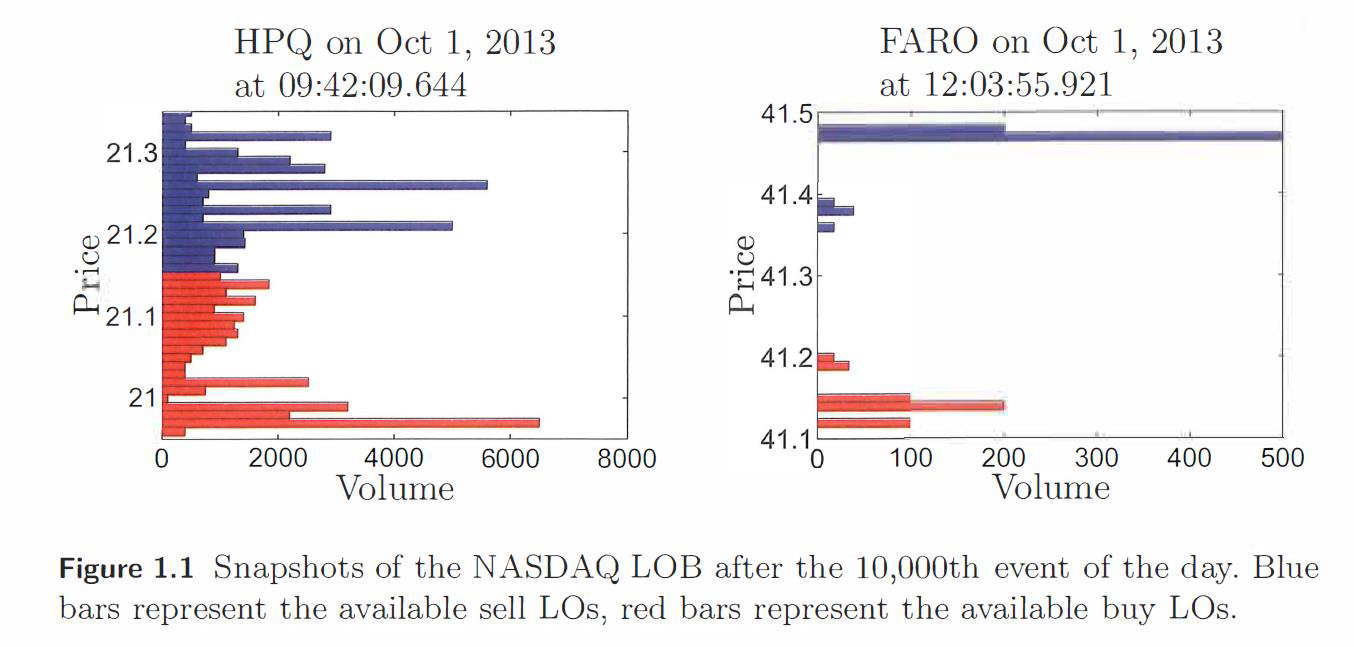
\includegraphics[width=\linewidth]{LOB.png}
\caption {La differenza tra un asset molto liquido e quindi con un volume alto di trade e uno poco liquido, il prezzo(non in figura) di HPQ è più vicino al suo midprice di quanto lo sia FARO}
\end{figure}

\newpage

%%%% NEWPAGE

\section{Il Limit Order Book}
\subsection{L'aggiunta di LO al LOB}
	in genere il LOB gestisce i LO con una coda FIFO per LO di prezzi uguali
\subsection{Microprice}
	ad ogni momento t può essere definito un MicroPrice di una stock come
\begin{center}
	{\emph{Microprice= ${\frac {V_t^b}{V_t^b + V_t^a}}P_t^a + {\frac {V_t^a}{V_t^b+V_t^a}}P_t^b$}}
\end{center}
	il microprice è una subdola misura della tendenza ad avvicinarsi al buy or sell order di una particolare stock

	con molti acquirenti il microprice tende ad avvicinarsi al prezzo di bid, e viceversa con molti seller.
\section{Tempo}
	\textbf{il ruolo del tempo è fondamentale} in un electronic exchange. \newline
	è necessario sistemare la propria posizione di trading in risposta ad ogni cambio o, addirittura, anticipandoli

	L'importanza della velocità è ciò che consente \textbf{L'high frequency trading}. \newline
	La velocità fa si che vengano sviluppati algoritmi di trading, influenzati a loro volta dalla scelta di:

	 linguaggi di programmazione,hardware,connessioni all'engine, utilizzo di ordini...\newline
	A loro volta gli exchange si adattano, creando nuovi tipi di ordine oltre ai MO e LO.

\newpage

%%%% NEWPAGE
\subsection{Tipi di ordine}
\begin{description}
	\item[Day Order] ordini che possono estendersi oltre le sessioni di mercato
	\item[Non-Routable] ordini che non possono estendersi oltre il mercato attuale
	\item[Pegged,Hide-not Slide] ordini basati su midpoint o sul prezzo nazionale
	\item[Hidden] ordini che non mostrano la loro quantità
	\item[Icebeg] ordini che mostrano una parte della loro quantità
	\item[Immediate-or-Cancel] eseguiti al prezzo migliore e poi cancellati (No walk-the-book)
	\item[Fill-or-Kill] ordini che vengono eseguiti UNICAMENTE al best price
	\item[Good-Till-Time] ordini con una spanna di tempo come life-time
	\item[Discretionary] ordini che mostrano un prezzo ma che in verità sono ad un altro prezzo (????)
\end{description}
	nella scelta dei nostri algoritmi dobbiamo essere a coscienza di ogni possibile tipo di ordine eseguibile non solo nel nostro exchange ma anche in tutti quelli che competono con noi.

\newpage

%%%% NEWPAGE
\section{Colocation}
	Gli exchange controllano quante e come le informazioni sono rilasciate,

	per una fee, possiamo ottenere più informazioni. \newline
	Oltre a questo offrono dei computer/server direttamente vicini all'engine per massimizzare la velocità delle nostre operazioni

	questo semplifica l'abilità di fornire servizi agli utenti e garantisce che ogni trader ha la stessa velocità di accesso e non sono svantaggiati rispetto a trader con hardware più potente

	ovviamente crea una distinzione tra trader colocati e non.
\section{Exchange Fees}
	un altro problema di cui bisogna essere allertati sono le exchange fee. \newline
	alcuni mercati impongono un \textbf{maker-taker system} che favorisce la liquidità degli asset

	fornendo una fee per i MO e dando un rebate,un pagamento, per i LO

	esistono invece mercati con una struttura inversa, dove è favorito chi toglie liquidità (I MO) \newline
	 questo è un grosso problema in quanto le fee distorgono(?) il prezzo di mercato
\section{Trader Class}
	Esistono 3 generiche classi di trader
\begin{description}
	\item[Fondamentale] sono guidati dai fondamenti dell'economia
	\item[Informato] guadagnano profitti dalle informazioni non riflettute sul market price, scambiando asset in anticipi
	\item[Market maker] professionali, che facilitano exchange in asset particolari
\end{description}
	Definiamo anche i \textbf{Proprietary traders}, traders che scambiano con vantaggi(reali e non) su traders più piccoli, questi 		vantaggi possono essere vari: conoscenza maggiore degli asset,identificare lo swing di un asset, conoscenza di pattern \newline
	gli \textbf{Investitori regolari} e i \textbf{Fondamentali} sono investitori che hanno un uso diretto degli asset scambiati

	sono individui che sperano di crescere insieme ad una corporazione, o persone che desiderano ribilanciare i loro investimenti

\subsection{Liquidità e traders}
	pensiamo ai trader \textbf{MarketMaker} come ad una tipologia passiva/reattiva che scambia utilizzando la loro profonda 			conoscenza del mercato ed in grado di adattarsi con le circonstanze. 
	
	Gli altri due tipi sono trader più aggressivi, che cercano di sfruttare specifiche informazioni ottenute all'infuori dell'ambiente di 		trading. \newline
	Fare mercato non equivale a generare liquidità cosi come trading informato non equivale a prendere liquidità.

	L'attività di Maket making in genere favorisce la liquidità, ma differenti strategie fanno si che questo non è sempre vero

	Viceversa, il trading informato non sempre avviene attraverso ordini aggressivi, ma è a volte meglio implementato attraverso

	ordini passivi che aggiungono liquidità invece che toglierla.

\chapter{Asset e ritorni}
	\section{Ritorni semplici ad un periodo}
	La maggior parte degli studi finanziari sono volti al ritorno, anziche il prezzo, degli asset.
\begin{description}
	\item[] Gli Asset return sono un resoconto completo e (scale-free?) delle opportunità di investimento di un investitore
	\item[] serie di ritorni sono statisticamente più interessanti di serie di prezzi
	\item[] vi sono diverse definizioni di asset return
\end{description}
Definiamo $P_t$ come prezzo di un asset in un periodo t(no dividendi). \newline
\subsection{Il periodo di Holding e i ritorni}
	Supponiamo l'acquisto di un asset a $t_0$ per $P_0$ e di venderlo a $t_1$ a prezzo $P_1$

	Supponendo l'assenza di dividendi tra i due periodi allora definiamo il rate of return come la variazione percentuale

	dei due prezzi:
\begin{center}
	$R(t_0,t_1)={\frac {P_1-P_0}{P_0}}$
\end{center}
	definiamo il tempo tra $t_0$ e $t_1$ come \textbf{holding period}  

	mentre $R(t_0,t_1)$ come \textbf{ritorni dell'holding period}.

	L\textbf{holding period} può essere un qualsiasi intervallo temporale.

\section{Ritorni semplici}
	definizione di \textbf{Ritorni lordi(?)}:

	il totale dei ritorni prima di dedurre qualsiasi fee o spesa necessaria, i ritorni lordi sono visti su uno specifico

	periodo temporale: un mese, un quadrimestre, un anno. 

	sono generalmente i ritorni promessi da, per esempio, una pubblicità. \newline
 	siano $P_t$ il prezzo nominale di un asset alla fine del mese t, che non paga divididendi

	$P_t-1$ il prezzo alla fine del mese t-1. \newline

\begin{center}
	{\emph{ritorni netti in un investimento tra t-1 e t}}= $R_{t-1,t}={\frac {P_t - P_{t-1}}{P_{t-1}}}= \%\Delta P_t$
\end{center}	
	che possiamo riscrivere come
\begin{center}
 	$1+R_{t-1,t}={\frac {P_t}{P_{t-1}}}$
\end{center}
	Il ritorno lordo di un mese è l'interpretazione del valore di {\EUR{1.00}} nell'asset per un mese.
\subsection{Esempio}
	Assumiamo di investire in un'azione Microsoft al periodo $t-1$ con $P_{t-1}$={\EUR{85}} e di venderla il mese successivo

	al prezzo $P_t$={\EUR{90}} allora
	
	i ritorni netti semplici di un mese e il lordo sono:
\begin{center}
	$R_t={\frac{90}{85}}-1 = 1,0588-1= 0,0588$ \newline
	$1+R_t = 1,0588$
\end{center}
	Abbiamo che il ritorno netto del mese è stato del 5,88\%

	oppure possiamo dire che l'investimento di 1 è cresciuto in 1,0588
\section{Ritorni compunded e Multi-Periodo} \footnote{check con Candelieri per la correttezza}
	definiamo che nel \textbf{periodo di k mesi} il ritorno semplice è nientemeno che il prodotto dei periodi mensili:

	\textbf{ritorno netto di un periodo k-simo}	$R_t[k]= {\frac{P_t-P_{t-k}}{P_{t-k}}} $

	\textbf{ritorno semplice di due mesi:}= ${\frac {P_t}{P_{t-2}}} - 1 $

	\textbf{il ritorno lordo su k mesi } è definito come il prodotto dei primi k-esimi ritorni lordi
\begin{center}
	${\prod\limits_{j=0}^{k-1}({1+R_{t-j}}})$
\end{center}
\subsection{Continous Compound Return}
	eseguendo  il \textbf{continuos compounding} su un asset possiamo computare facilmente i ritorni

	su un periodo di tempo
\begin{center}
	$\log{(1+R_t)} = r_t =\log{({\frac {P_t}{P_{t-1}}})}$
\end{center}
	per un periodo di tempo k
\begin{center}
	$r_t[k]= \log{(1+R_t[k])} =\log{[(1+R_t)(1+R_{t-1})  ...(1+R_{t-k+1})]}$
\end{center}
\subsection{Esempio}
	ritornando all'esempio precedente con
	\begin{center}
	$P_t$ = 90  \\
	$P_{t-1}$ = 85 \\
	$P_{t-2}$ = 80 \\
	\end{center}
	allora il ritorno per due mesi è:
	\begin{center}
	$R_t(2) = {\frac {90-80}{80}} - 1 = 0,1250 $
	\end{center}
	che equivale al 12.50\% per due mesi

	che equivale a sua volta al prodotto tra i due ritorni ad un mese:
	\begin{center}
	$R_{t-1}= {\frac {85-80}{80}} - 1 =1,0625-1= 0,0625 $\\
	$R_t = {\frac {90-85}{85}} - 1 =1,0588-1= 0,0588 $ \\
	 il cui prodotto:  $1,0625*1,0588=1,1250 = 12,50\% $ 
	\end{center}
\section{Ritorni e Portfolio}
	Consideriamo un investimento di valore V\$ su due asset A e B.

	sia $x_A$ e $x_B$ la frazione di V che i due asset rappresentano,

	questo valore è definito \textbf{investment share}

	sappiamo che il valore in dollari è rappresentato da $V*x_A$ e $V*x_B$

	assumiamo che la somma degli \textbf{investment share} $x_A + x_B$ = 1. \newline
	un insieme di \textbf{investment share} definisce il portfolio,
	quando i valori degli investment share sono negativi siamo in short selling.
\subsection{Simple Returns}
	definiamo $R_{A,t}$ e $R_{B,t}$ come i ritorni semplici mensili degli asset A e B

	vogliamo definire i ritorni del portfolio p definito da ($x_A,x_B$) \footnote{Per dimostrazioni vedi slide}

\begin{center}
	$R_{p,t} = x_A R_{A,t} + x_B R_{B,t}$
\end{center}
\section{I dividendi}
	assumendo che un dato asset paghi dividendi tra t-1 e t  abbiamo il valore dei dividendi al tempo t: $D_t$
	
	allora il calcolo dei ritorni diventa:

\begin{center}
	$R_t^{total} = {\frac{P_t + D_t - P_{t-1}}{P_{t-1}}}$ = ${\frac {P_t - P_{t-1}}{P_{t-1}}}$
	\marginpar{Capital gains e Dividendi} + ${\frac {D_t}{P_{t-1}}}$
\end{center}
 	definiamo i \textbf{capital gain}: guadagno in capitale: identifica il guadagno ottenuto dalla compravendita di strumenti finanziari,

	è la differenza tra prezzo di acquisto e di vendita di uno strumento finanziario.

	è tassato. \newline
	Se un asset paga dividendi periodici la definizione dei ritorni di un asset è modificata in
\begin{center}
	$1+R_t^{total}= {\frac {P_t + D_t}{P_{t-1}}} $
\end{center}

\section{Inflazione}
	I calcoli sui ritorni finora effettuati sono considerati \textbf{nominali} o prezzi attuali degli asset

	I ritorni calcolati su prezzi nominali sono detti \textbf{ritorni nominali} \newline
	I \textbf{veri} ritorni su un asset in un \textbf{horizon} considerano la crescita dei prezzi su quell'horizon (?)
	
	se il nominal price cresce più in fretta del prezzo generico allora i ritorni nominali saranno maggiori dell'inflazione,
	
	 ed il nostro ritorno reale sarà positivo

	Viceversa se cresce più lentamente il nostro ritorno sarà negativo in quanto il valore dei ritorni sarà minore dell'inflazione. 		\newline
	La \textbf{computazione dei ritorni reali} è un processo a due step:
\begin{enumerate}
	\item De-inflaziona il prezzo nominale con il prezzo generico
	\item Computa i ritorni semplici sul prezzo De-inflazionato
\end{enumerate}
\subsection{Calcolo per i ritorni reali}
	siano $P_t$ il prezzo nominale di un asset al tempo t e $CPI_t$ un indice del prezzo generico.
	
	alora il prezzo reale al tempo t sarà
\begin{center}
	$P_t^{real} = {\frac {P_t}{CPI_t}}$	
\end{center}
	una volta ottenuto il prezzo reale sarà possibile calcolare i ritorni come al solito. 
\subsection{Calcolo Inflazione}
	Possiamo anche definire l'inflazione al tempo t come:
\begin{center}
	$\pi_t = \%\Delta CPI_t = {\frac {CPI_t - CPI_{t-1}}{CPI_{t-1}}} $ \\
	$R_t^{Real}= {\frac {1+R_t}{1+ \pi_t}} - 1 $ 
\end{center} 
\newpage

%%%% NEWPAGE
\section{Ritorni annuali}
	In genere convertiamo i ritorni in ritorni annuali per stabilire delle basi per effettuare confronti:
	Compound Annual Gross Return(CAGR), o Ritorni annuali Lordi,

	Compound Annual net Return(CANR), o Ritorni annuali Netti\footnote{non utilizziamo $R_A$ = 12$R_m$ perchè assumiamo ritorni compounded}
\begin{center}
	$CAGR = 1+R_A = 1+R_T(12) = (1+R_m)^{12} $ \\
	$CANR = R_A = (1+R_m)^12 - 1 $ \\
\end{center}
\subsection{Esempio}
	Supponiamo che $R_t$ per una stock Microsoft sia 5,88\%.

	se assumiamo vero questo ritorno per 12 mesi allora l'annuale è: \newline
	$R_A = (1,0588)^12 - 1 = 1,9850 - 1 = 0,9850 $ 

	oppure 98,50\% annuale.
\section{Ritorni medi}
	Per un investimento su un dato horizon, ci interessa computare la misura dei ritorni medi su quell'horizon

	consideriamo una sequenza di investimenti mensili su un anno con ritorni mensili abbiamo due possibilità
\begin{enumerate}
	\item Media Aritmetica: $ \bar{R} = {\frac {1}{12}}(R_1 + R_2 ... + R_12) $ che può essere errata
	\item Media Geometrica: $(1+ \bar{R})^{12} = (1+R_A) = (1+R_1)(1+R_2)...(1+R_{12}) $

		$ \bar{R} = (1+R_A)^{\frac {1}{12}} - 1$

		$ =[(1+R_1)(1+R_2)...(1+R_{12})]^{\frac{1}{12}} - 1$ che è più precisa

\end {enumerate}

\section{Annualizzare i ritorni}
	In genere differenti horizon sono annualizzati: convertiti in ritorni annuali per confrontarli con altri investimenti. \newline
	Il processo di annualizzazione dipende dall'holding period dell'investimento e da una assunzione sul compounding.

 	Questo è un processo semplice per horizon annuali, ma richiede di fare assunzioni particolari su periodi più brevi:

	Avrò lo stesso ritorno $R_t$ per ogni periodo dell'anno? allora possiamo utilizzare le formule per il netto e il lordo precedenti.
 \newpage
  
\chapter{Ottimizzazione Portfolio}
	nel 1952 viene presentata da \textbf{Markowitz Harry} le basi per selezionare un portfolio:

\begin{center}
	{\emph{Una combinazione di asset che in un dato periodo di tempo produce ritorni maggiori ad un mischio minore}}
\end{center}

	vi sono due step da seguire:
\begin{enumerate}
	\item Identificare la combinazione di asset ottimali rispetto a \textbf{rischio e ritorno} attesi per creare un portfolio
	\item Scegliere il miglior portfolio che rispecchia la \textbf{funzione di utilità dell'investitore}
\end{enumerate}
	La \textbf{funzione di utilità dell'investitore} riguarda limiti,tolleranza al rischio,tipologia e numero di asset desiderati e

	capitale totale disponibile.
\newpage

%%%% NEWPAGE
\section{Il modello media-varianza}
	Dalla ipotesi di Markowitz per la selezione del modello deriviamo che:

	I ritorni attesi sono "\textbf{buoni}"

	La varianza, nei ritorni attesi sono da \textbf{evitarsi}. \newline
	Cerchiamo di dimostrare matematicamente l'importanza nella \textbf{diversificazione del portfolio}. 
\subsection{Reminder sui Portfolio return}
	In genere, per un dato portfolio di n asset con investment share $x_i$ tale che $x_1+x_2...+x_n = 1$ abbiamo che
\begin{center}
	$1+R_{p,t} = \sum\limits_{i=1}^n x_i(1+R_{i,t}) $\\
	$R_{p,t} =  \sum\limits_{i=1}^n x_i R_{i,t}= x_1 R_{1t}+... + x_n R{nt}$
\end{center}

	Definiamo a questo punto il \textbf{Valore Medio} o \textbf{Valore atteso} ad un tempo \textbf{t} di un portfolio \textbf{w} E la sua varianza \footnote{ $\rho =$ coefficente di correlazioene tra due asset}
\begin{center}
	$\mu_w = E(R_t^w) =  \sum\limits_{i=1}^N w_i E(R_{i,t}) $ 
	$\sigma_w^2 = Var(R_t^w) =  \sum\limits_{i=1}^N  \sum\limits_{j=1}^N w_i w_j \sigma_i \sigma_j \rho_{i,j} =  \sum		\limits_{i=1}^N  \sum\limits_{j=1}^N w_i w_j \sigma_i \sigma_j  $ 
\end{center}
\subsection{Considerazioni}
	\textbf{Caso 1} il ritorno di N asset su un portfolio è incorrelato a coppie:

	\emph{Maggiore è il numero di asset incorrelato, minore è il rischio del portfolio}. 

	\textbf{Caso 2} i iritorni degli asset di un portfolio sono correlati: 

	\emph{Maggiore è la presenza di asset correlati, maggiore è il rischio che vi sia un rischio comune a tutti gli asset}. \newline

	Pertanto, la \textbf{diversificazione} è ottenuta considerando \textbf{asset altamente incorrelati}.

	Plottando un portfolio dato da una funzione N abbiamo che circa 15-20 asset incorrelati sono un numero ragionevole.

\newpage

%%%% NEWPAGE
\section{Portfolio a Rischio minimo}
	Essendo che secondo la regola di Markowitz gli investitori sono concentrati sull'ottenimento di benefit con il minor rischio 			possibile,

	La selezione di un portfolio di Markowitz si riduce a:
\begin{center}
	\emph{ Trova i pesi  $w=(w_1,w_2,w_3,...,w_N)$ tali che, per un tasso di ritorno $r^*$, il portfolio \textbf{w} ha ritorni 		$r^*$  con varianza minimale }
\end{center}
	La varianza minima per un dato portfolio si collega ai problemi di ottimizazione: \footnote{Candelieri? w'}
\begin{center}
	$ \underset{w}{min}$ $ w' Cw $ \\
	soggetto a: $ w' \mu = r^* $ \\
 	e tale che $ \sum\limits_{i_1}^{N} w_i=1 $
\end{center}
	questo è un problema Quadratico con vincoli lineari, questo può essere ridotto a un sistema lineare. \footnote{Lagrangiane}

	I vincoli indicano che l'nvestitore utilizza tutto il suo budget per gli N asset
\subsection{Considerazioni}
	Il modello non impone restrizioni sui valori dei pesi (possono essere long o short)

	Sotto queste condizioni e senza arbitraggio, il problema può essere risolto con i \textbf{Lagrange Multipliers}

	Una volta risolto il sistema lineare otterremo i pesi dei singoli w con una media \textbf{r*} e varianza minima.

	Questa soluzione è detta \textbf{efficiente} in quanto è IL portfolio con ritorni attesi r* e varianza minima rispetto ad altri 			portfolii con lo stesso valore atteso.
\section{Frontiera di efficienza}
	Per un insieme di N assets che costituiscono un portfolio, vanno considerati i possibili \textbf{problemi quadratici} per 			ottenere
	una definizione efficiente dei pesi w. \newline

	da questi pesi otteniamo la deviazione standard del portfolio w:
\begin{center}
	$\sigma^*=std(R^{w*})=\sqrt{(w^*)'Cw*}$
\end{center}
	%%%%
\begin{figure}[h]
  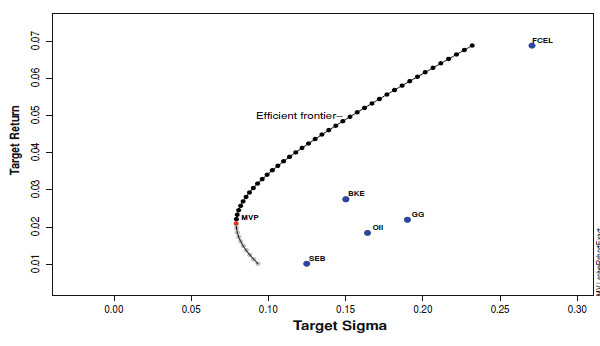
\includegraphics[width=\linewidth]{EfficientFrontier.png}
  \caption{Frontiera di efficienza}
  \label{fig:EfficientFrontier}
\end{figure}
	%%%%	

\newpage

%%%% NEWPAGE
\section{Portfolio con asset risk-free}
	Fino ad ora abbiamo assunto che tutti gli asset che utilizziamo nel nostro portfolio presentino dei rischi

	L'aggiunta di risk-free asset \footnote{bond} causa delle consequenze.
	Queste sono la consapevolezza di prestare \footnote{essere prestati} denaro ad un interesse conosciuto $r_0$ e con 0 rischio:
	
	Prestare denaro significa avere un asset risk-free con un peso w positivo

	Ricevere denaro significa avere un asset risk-free con un peso w negativo. \newline
	Sia $r_f=r_0* \tau$ la rata risk-free,o ritorno, nel periodo di tempo $\tau$.

	Un portfolio che consiste solo di questo asset ha valore medio $r_f$ e varianza 0.

	Il rischio di questo portfolio nel piano \emph{rischio-media} è nel punto(0,$r_f$).
	ri-considerando le formule per calcolare il valore di un portfolio dato da
\begin{center}
	$\mu_w = E(R_t^w) =  \sum\limits_{i=1}^N w_i E(R_{i,t}) $ 
	$\sigma_w^2 = Var(R_t^w) =  \sum\limits_{i=1}^N  \sum\limits_{j=1}^N w_i w_j \sigma_i \sigma_j \rho_{i,j} =  \sum		\limits_{i=1}^N  \sum\limits_{j=1}^N w_i w_j \sigma_i \sigma_j  $ 
\end{center}
	sia allora $w_f$ il peso dell'asset risk free nel portfolio, abbiamo che
\begin{center}
$	1-w_f=w_1+...+w_N$
\end{center}
	questo vale a dire che l'investimento totale è diviso in due parti: la risk-free e la non risk-free.
	vediamo il portfolio come una coppia (w,$w_f)=(w_1,w_N,w_f) $ che consiste di un asset risk-free, di media $r_f$
	e con deviazione standard 0, insieme al vettore degli N asset rischiosi, con peso 1-$w_f$, media $\mu_w$ e deviazione $			\sigma_w$. \newline
	\textbf{NOTA come la covarianza di questi è sempre 0}. \newline
	a questo punto il portfolio combinato $\omega$=(w,$w_f$) ha:
\begin{center}
	valore atteso $\mu_\omega = w_f r_f+(1-w_f)\mu_w $ \\
	deviazione standard $\sigma_\omega = (1-w_f) \sigma_w$
\end{center}

	vediamo in queste equazioni come media e deviazione del portfolio dipendano linearmente da $w_f$. pertanto

	variando il valore di $w_f$ otterremo che i diversi portfolii rappresentati dalle equazioni sono una linea retta con origine in

	(0,$r_f$) passante attraverso i punti ($sigma_w,mu_w$) nel piano rischio-media. \newline
	Inoltre, modificando i pesi dei N asset rischiosi costruiamo un altro portfolio \textbf{w'},  che combinato con il risk-free asset
	genera un altra linea retta di tutti i possibili portfolii creati da queste combinazioni. \newline

	Concludiamo quindi che la regione ammissibile dei portfolii Markowitziani(o della regione media-varianza) ottenuti con:
	N asset rischiosi,
	1 asset risk-free.
	è un triangolo con un vertice nel punto rappresentante l'asset risk-free e che copre tutta l'iperbole contenente tutti i possibili 		portfolii. 
	%%%% IMMAGINE EFFICIENTFRONTIER_TRIANGOLO
\begin{figure}[h]
  	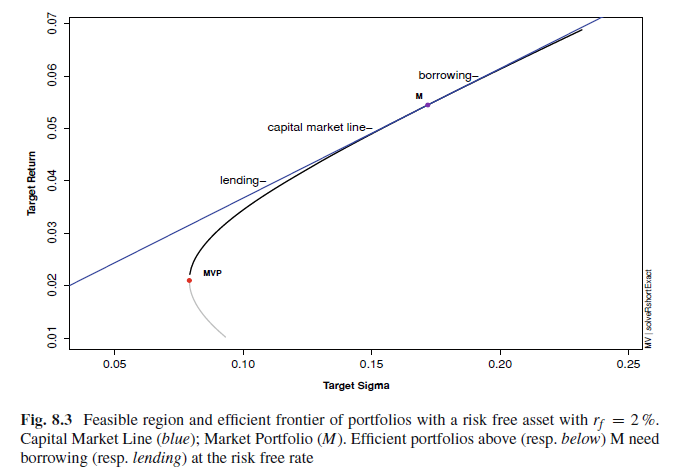
\includegraphics[width=\linewidth]{EfficientFrontier_Triangle.png}
%  \caption{}
	  \label{fig:EfficientTriangle}
\end{figure}
%%%
	\newpage

%%%% NEWPAGE
\section{La linea del mercato capitale e il portfolio di mercato}
	La frontiera di efficienza è adesso una linea retta con intercetta in (0,$r_f$) 

	e tangente alla frontiera di efficienza dei portfolii rischiosi \footnote{ da ora chiamati $EF_r$} nel piano rischio-media. \newline
	La tangente che descrive i portfolii è definita \textbf{Capital Market Line(CML)}, il punto in cui CML  incontra $EF_r$ ha:

	coordinate della deviazione standard e valore atteso di un portfolio particolare: il \emph{Market Portfolio}.
\subsection{Market Portfolio}	
	Il \emph{Market Portfolio} è il miglior portfolio con rispetto al rapporto ${\frac{excess return}{rischio}}$ \newline
	esso è la miglior rappresentazione del mercato, in quanto contiene ogni azione sul mercato in propororzione al loro peso. \newline
	sia $\theta$ l'angolo tra l'asse orizzontale e una linea passante su(0,$r_f$) e un punto ($std(R^w),E(R^w)$), corrispondente    	 a un qualche portfolio rischio so allora:
\begin{center}
 $\tan{\theta} = {\frac {E(R^w) - r_f}{std(R^w)}} $
\end{center} 
	il \textbf{Market Portfolio} è il punto che massimizza $\tan{\theta}$, questo da la inclinazione della CML computata al punto di tangenza della frontiera rischiosa di efficienza  \footnote{Candelieri(??)}.

	Dall'equazione vediamo che il MarketPortfolio da il massimo rapporto (ritorno/rischio); i pesi di tale soluzione massimizzano 
	$\tan\theta$ e sono in proporzione al loro peso sul mercato.

\newpage
%%%% NEWPAGE
\subsection{Sharpe Ratio}
	Sia ($std(R_m), E(R_m)$) il punto che descrive il Market Portfolio, il punto di tangenza tra CML e E$F_r$ \newline
	Come prima,($0,r_f$) rappresenta l'asset risk-free. Allora ogni punto ($std(R^w),E(R^w)$) nella CML, ogni portfolio efficiente è tale che: 
\begin{center}
	$E(R^w)= w_f r_f + (1-w_f)E(R_M) $ \\
	$std(R^w)=(1-w_f)std(R_M) $ \\
\end{center}
	dove $w_f$ è una frazione dell'investimento sul risk-free asset: 

	\emph{ se $w_r \geq 0 $ stiamo prestando con un tasso di interesse risk-free; se $w_r \leq 0 $ stiamo ricevendo un prestito 
	con un tasso risk-free, Per aumentare i nostri investimenti sugli asset rischiosi }
	 \newline
	Possiamo riscrivere CML come:
\begin{center}
	$E(R^W)$ =$ r_f+(1-w_F)(E(R_M)-r_f)$ \\
	 = $r_f+{\frac{(E(R_M)-r_f)}{std(R_M)}}std(R^W)$
\end{center}
 	definiamo, in queste equazioni la \textbf{Sharpe Ratio} del Market Portfolio come $SR_M={\frac{(E(R_M)-r_f)}{std(R_M)}}$  \newline
	In genere, per un qualunque portfolio la \textbf{Sharpe Ratio} è il numero:
\begin{center}
	$SR^W={\frac{(E(R^W)-r_f)}{std(R^W)}}$
\end{center}
	Essa rappresenta la misura di un portfolio di premiare il tasso di variabilità \footnote{Candelieri, non varianza?}. \newline
	Più alta la Sharpe Ratio, migliori gli investimenti, con il limite superiore di una qualunque Sharpe Ratio individuata nel Market 
	Portfolio. 

	Dunque, per ogni portfolio veramente efficiente, con almeno un risk-free asset, abbiamo che 
\begin{center}
	$SR^W = SR_M$
\end{center}
	è sempre vera.  \newline
	Riassumendo, in un mondo basato sulla media-varianza MarkoWitziana, il meglio che si può fare è: \newline
	 allocare  una porzione dell'investimento in UN  asset risk-free, e tutto il resto nel Market Portfolio, \newline
	garantendo cosi il miglior rapporto di ritorno/variabilità. 

\newpage
%%%% NEWPAGE
\section{Il modello Capital Asset Pricing e Beta}
	La Capital Market Line, CML, mostra l'equilibrio tra valore atteso e deviazione standard in un portfolio efficiente. \newline
	è desiderabile avere un equilibrio simile tra rischio e reward di un asset rischioso rispetto al portfolio in cui voglio inserirlo. \newline
	L'equilibrio tra asset e un portfolio è dato dal \textbf{CAPM} \emph{Capital Asset Pricing Model}.
\begin{theorem}[Teorema CAPM]
	Sia $E(R_M)$ i ritorni attesi del \emph{Market Portfolio}, $\sigma_M = std(R_M)$ la sua deviazione standard, e $r_f$ il risk-free return in un periodo di tempo $\tau$ \newline
	Sia $E(R_i)$ il valore atteso di un asset i, $\sigma_i$ la sua deviazione standard, e $\sigma_{iM}=CoV(R_i,R_M)$ la covarianza tra $R_i$ e $R_M$

	allora:
\begin{center}
	$E(R_i)=r_f+\beta_i (E(R_M)-r_f)$ \\
	$ \beta_i= {\frac {\sigma_{iM}}{\sigma_M^2}} = {\frac {Cov(R_i,R_M)}{Var(R_M)}} $
\end{center}
\end{theorem}
	il CAPM fa si che il valore atteso di ritorno dell'asset i, $E(R_i)-r_f$, conosciuto anche come il premio del rischio, è proporzionale  \newline
	di un fattore $\beta_i$ ai valori attesi di ritorno del Market Portfolio, $E(R_M)-r_f$ o il premio del market. \newline
	Il coefficiente $\beta_i$ anche conosciuto come \emph{beta dell'asset i} è la percentuale del premio dell'asset sul premio del market.
\subsection{CAPM come modello di pricing}
	Supponendo di voler sapere il prezzo P di un asset il cui payoff dopo un periodo $\tau$ è un valore casuale $P_\tau$ \newline
	Allora il rate di ritorno dell'asset in un periodo $\tau$ è $R_\tau = (P_\tau /P) - 1$,
	
	per CAPM il valore atteso $R_\tau$ è relativo al rate di ritorni del mercato nello stesso periodo di tempo.
\begin{center}
	$E(R_\tau)={\frac {E(P_\tau)}{P}}-1 = r_f + \beta(E(R_M)-r_f) $ \\
	con $\beta$ beta dell'asset che stiamo analizzando
\end{center}
	risolvendo per P otteniamo
\begin{center}
	$P= {\frac {E(P_\tau)}{1+r_f+\beta(E(R_M)-r_f)}} $
\end{center}
 	che è una generalizzazione della formula del discounted cash flow per asset risk free, includendo asset rischiosi.
\subsection{Il significato di Beta}
	Formalmente, il beta di un asset rappresenta la dipendenza lineare dei ritorni dell'asset e dei ritorni del mercato in proporzione alla volatilità del mercato:
\begin{center}
	\Large{$ \beta_i = {\frac {Cov(R_i,R_M)}{Var(R_M)}} = \rho(R_i,R_M){\frac {\sigma_i}{\sigma_M}}$}
\end{center}
	utilizzando l'equazione precedente possiamo ottenere delle interpretazioni dei valori di un asset come misura di un suo movimento con il mercato:

	Sia $\beta=\beta_i$ e $\rho=\rho(R_i,R_M)$ il coefficiente di correlazione dell'asset e il mercato:
%%%IMMAGINE VALORE BETA
\begin{figure}[h]
  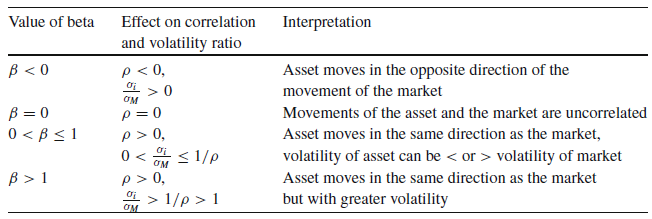
\includegraphics[width=\linewidth]{MeaningOfBeta.png}
 % \caption{}
  \label{fig:beta}
\end{figure}
%%%
	ad esempio, supponendo che \textbf{ $\beta=0$} significa che asset e mercato non hanno relazioni,\newline
	essendo che  la deviazione standard è sempe positiva.

	In questo caso, secondo il CAPM: $E(R_i)=r_f$, il rischio del premio è zero. \newline
	 un altro caso è $\beta > 1$ \newline
	Questo implica che il mercato e l'asset sono positivamente correlato, ed il rischio dell'asset è maggiore del rischio del mercato.

	Da questo rischio extra deduciamo con CAMP: $E(R_i)>E(R_M)$, l'asset potrebbe battere il mercato.\newline
\subsection{Continuo sull'interpretazione di Beta} \footnote{Totalmente non compreso}
	La nostra interpretazione è una delle molte interpretazioni;

	L'uso più comune di Beta è la misurazione del rischio relativo al mercato. ma è uno solo dei fattori dell'equazione \newline %%%da finire
\subsection{Stimare il  valore di Beta}
	Date n coppie di stock i, $R_i$ e di mercato, $R_m$ in un periodo di tempo uguale, possiamo stimare il beta di i con rispetto al mercato utilizzando degli stimatori per la covarianza e la varianza:
\begin{figure}[h]
  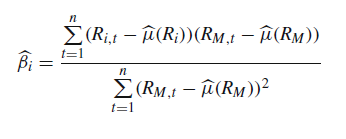
\includegraphics[width=\linewidth]{TheBigBetaFormula.png}
 % \caption{}
  \label{fig:betaformula}
\end{figure}	
	\newline per questo stimatore assumiamo che il rate della risk free $r_f$ rimanga costante durante il periodo
	

\end{document}